% !TeX root = Report.tex
\section{Literature Review}

\subsection{Routing in Sensor Networks}
Wireless sensor networks can typically contain hundreds or thousands of nodes, with so many devices communicating with each other it is very important to develop robust routing techniques designed specifically for these networks. The algorithms that have been developed trace their origins from traditional distributed computation protocols such as flooding, tree aggregation and clustering;  However, these new protocols are designed, first and foremost, to address the primary constraints of wireless sensor network.   

\subsubsection*{Flooding and Gossiping}
Flooding and Gossiping are arguably the most simplistic routing algorithms available to a wireless sensor network developer. In flooding, wireless sensor network nodes broadcast to all their neighbours any messages that they receive, messages only stops when either i) the packet arrives at its intended recipient or ii) the messages maximum number of node hops is reached. Gossiping is similar to flooding in many ways, the only difference being when a node receives a message instead of broadcasting it to every neighbour the node randomly picks one neighbour to forward the message too. Due to the simplicity of Flooding and Gossiping there is no need for any complex routing algorithms or topology maintenance \cite{Akkaya2005325}. However, these two routing algorithms do suffer from several drawbacks, these are: \emph{Implosion} - is when the same message is sent to the same recipient twice (Gossiping avoids this but causes delays in the propagation of messages through the network), \emph{Overlap} - is when two nodes sense the same change in a local environment and both send similar messages to the same neighbour and \emph{Resource Blindness} -  is when the routing algorithm consumes large amounts of energy with no consideration for efficiency \cite{Akkaya2005325}. Sensor Protocols for Information via Negotiation (SPIN) is a family of routing algorithms designed to address the issues with traditional Flooding and Gossiping protocols\cite{TankBible, Akkaya2005325}. The family does this by using data negotiation and resource-adaptive algorithms, for example nods running SPIN have access to the current battery level of the node and uses this information to adapt the protocol based on how much energy is remaining. Additionally, the SPIN family of protocols uses the concept of meta-data to reduce the level of redundant data sent around the network.

\subsubsection*{Clustering}
Clustering is a form of hierarchical routing that has a long history of improving the efficiency of networks, originally it was used to find the optimal placement of logic gates in digital circuits \cite{clustering}. Both in these applications and more modern variations the basic principle of clustering remains the same, to group (in a logical way) nodes of a network according to their (typically geographic) locality \cite{1628365}. Each node in one of these \emph{clusters} has a single point of contact with the rest of the network, in a wireless sensor network this is a specific node in each cluster known as the cluster head (CH). The cluster heads then communicates with each other and the base station to route packets around the network. The benefit of clustering a network is in reducing global network traffic, in a clustered network each node need only route messages to its CH rather than all the way to its destination. In some applications the CH can perform data aggregation or compression function\cite{1285913, aggregation} on the messages it forwards to reduce traffic between clusters; The nature of these functions is always application-specific. However, the nature of clustering means that a cluster head has a significantly higher workload than any other node in its cluster, it must listen to every message sent from the cluster and possibly forward just as many to the other cluster heads in the network. In domains where nodes do not have permanent power source (such as WSNs), this leads to greater energy usage, causing CH batteries to drain faster\cite{placement}. As a result of this, many modern clustering algorithms (e.g. \cite{eemc, secc}) rely on or take inspiration from the Low Energy Adaptive Clustering Hierarchy (LEACH) \cite{LEACH}.

LEACH and LEACH-C are two clustering algorithms proposed by \citeauthor{LEACH}, in their paper the authors showed that the standard LEACH protocol performed significantly better than static clustering in terms of energy efficiency, with LEACH-C performing better still. However, the inclusion of both rounds and TDMA in LEACH means that it requires nodes in a WSN to be synchronised, which comes with significant implications in terms of operational complexity. LEACH itself offers no solutions either towards ensuring that nodes maintain synchronisation, or towards detecting if some nodes (or more likely, an entire cluster) is not performing correctly due to slipping from the prescribed TDMA schedule. However, the authors themselves suggest that a possible improvement to negate the need for TDMA is some event-based method for applications in which nodes do not generate transmissible data constantly or at prescribed intervals.

\subsubsection*{Tree Aggregation}
Tree aggregation is another hierarchical routing protocol, this algorithm differs from clustering in that it divides a network into a tree structure with the root node situated at the base station. Nodes that are furthest from the base station (in hops) become leaves of the tree and any intermediate nodes become branches. Leaves and branches forward messages towards the base station and around the network using the tree structure, this results in a reduced number of global network messages over other algorithms such as flooding. The message count can be further reduced in a similar way to clustering, by implementing a data aggregation or compression function at each branch node of the network. The drawbacks of tree aggregation are clearly similar to clustering i) branch nodes have a higher workload than leaf nodes ii) if a branch nodes battery is depleted and the node turns off it can leave entire section of the network that it connects with the base station disconnected. There are several prominent tree aggregation algorithm (such as TAG, MFS and DCTC \cite{1628365}). Although very similar, they all take differing approaches to organising the data aggregation process of the branch nodes in order to reduce collisions and therefore messages in the network. For example, TAG uses the idea of a periodic traffic pattern which is divided into time intervals for each layer of the tree, this ensures that each branch receives as many messages from its children as possible before it forwards to the next layer.   


\cite{aggphdfeng} % THESIS
\cite{TankBible} % SURVEY ON ROUTING TECHNIQUES
\cite{Akkaya2005325} % SURVEY ON ROUTING TECHNIQUES

\subsection{Simulating Sensor Networks}

\subsubsection*{Contiki}
% Cite basically all the papers at: http://www.contiki-os.org/support.html

\paragraph{A Database In Every Sensor} 
\cite{Tsiftes:2011:DS:2070942.2070974} %http://dunkels.com/adam/tsiftes11database.pdf
\cite{TinyDB}


%\paragraph{Sensor Network IP Stacks} -- Not really need, IP work done in RIME
%\cite{ko2011beyond} % http://dunkels.com/adam/ko11beyond.pdf
%\cite{dunkels2009efficient} % http://dunkels.com/adam/yazar09efficient.pdf
%\cite{Durvy:2008:MSN:1460412.1460483} %http://dunkels.com/adam/durvy08making.pdf
%\cite{Dunkels:2003:FTA:1066116.1066118} % http://dunkels.com/adam/mobisys2003.pdf

%Bring into interoperability with the Internet of Things
\cite{Christin_Reinhardt_Mogre_Steinmetz_2009}

\paragraph{Cooja / MSPSim}
\cite{Eriksson:2009:CIT:1537614.1537650} % https://dl.acm.org/citation.cfm?id=1537614.1537650

\paragraph{Protothreads}
\cite{Dunkels:2006:PSE:1182807.1182811} % http://dunkels.com/adam/dunkels06protothreads.pdf

\paragraph{Energy Estimation}
\cite{Dunkels:2007:SOE:1278972.1278979} % http://dunkels.com/adam/dunkels07softwarebased.pdf

\paragraph{RIME and IP Stacks}

TCP/IP is traditionally viewed as unsuitable in sensor networks, \citeauthor{Estrin:1999:NCC:313451.313556} suggested that sensor networks have such different requirements to traditional networks, and that the overall structure of these networks needs to be reconsidered \cite{Estrin:1999:NCC:313451.313556}. Some of the problems \citeauthor{Estrin:1999:NCC:313451.313556} associated with IP in sensor networks included \cite{Estrin:1999:NCC:313451.313556}:
\begin{itemize}
	\item ``The sheer numbers of these devices, and their unattended deployment, will preclude reliance on a broadcast communication or the configuration currently needed to deploy and operate networked devices.''
	\item ``Unlike traditional networks, a sensor node may not need an identity (e.g., an address).''
	\item ``Traditional networks are designed to accommodate a wide range of applications.''
\end{itemize}
\citeauthor{Hui:2008:IDL:1460412.1460415} suggested that these problems are largely due to IPv4 and not the later IPv6 stating ``IPv6 is better suited to the needs of WSNs than IPv4 in every dimension'' \cite{Hui:2008:IDL:1460412.1460415}, further showing that a IPv6 based network architecture could be used in sensor networks, and provides a strong foundation in which to base further work \cite{Durvy:2008:MSN:1460412.1460483}. Simplified versions have been suggested as well as optimisations performed with headers \cite{Dunkels:2003:FTA:1066116.1066118,Dunkels04makingtcp/ip}, but they still had issues with regards to being based on IPv4.  \citeauthor{Estrin:1999:NCC:313451.313556} implementation of an IPv6 based architecture still had some problems, such as large headers, and the reliance on routing tables. The implementation had many benefits when concerning applications involving Neighbour Discovery and routing, but provided little improvements towards applications not involving identities (such as Flooding).

\citeauthor{Dunkels:2007:ACA:1322263.1322295} developed a common architecture, which allowed for much more code reuse and interoperability between protocols, this involved the RIME communication stack. The need for this new layer was brought about from applications needing to run over multiple protocols, leaving them unable to rely on specific communication mechanisms (such as retransmissions and acknowledgements) \cite{Dunkels:2007:ACA:1322263.1322295}. Previous work by \citeauthor{Ee:2006:MNL:1298455.1298479,Polastre:2005:ULA:1098918.1098928} \cite{Ee:2006:MNL:1298455.1298479,Polastre:2005:ULA:1098918.1098928} did not effectively solve the problem of protocols running on top of the lower layers, but did provide a basis for the RIME stack \cite{Dunkels:2007:ACA:1322263.1322295}. 

The RIME communication stack presents a solution to the cross-layer information-sharing problem of a layered communication stack by separating the protocol logic from the details of the packet headers. Packet headers need to be small, yet adaptive enough to encompass any type of communications. They solved this by using the notion of Packet Attributes. Modules would be used to transform data and the attributes into the corresponding packets (with headers and payloads). This provides the developer access too lower level information, without violating layering principles, yet with similar execution performance. This also allows interoperability with all protocols, abstracting the networking layers from the main application layer. For the application layer, RIME provides many communication primitives (such as Single-Hop Broadcasting) \cite{Dunkels:2007:ACA:1322263.1322295}, these primitives were selected based on analysis on the common use cases in WSNs.

\begin{figure}[H]
	\centering
	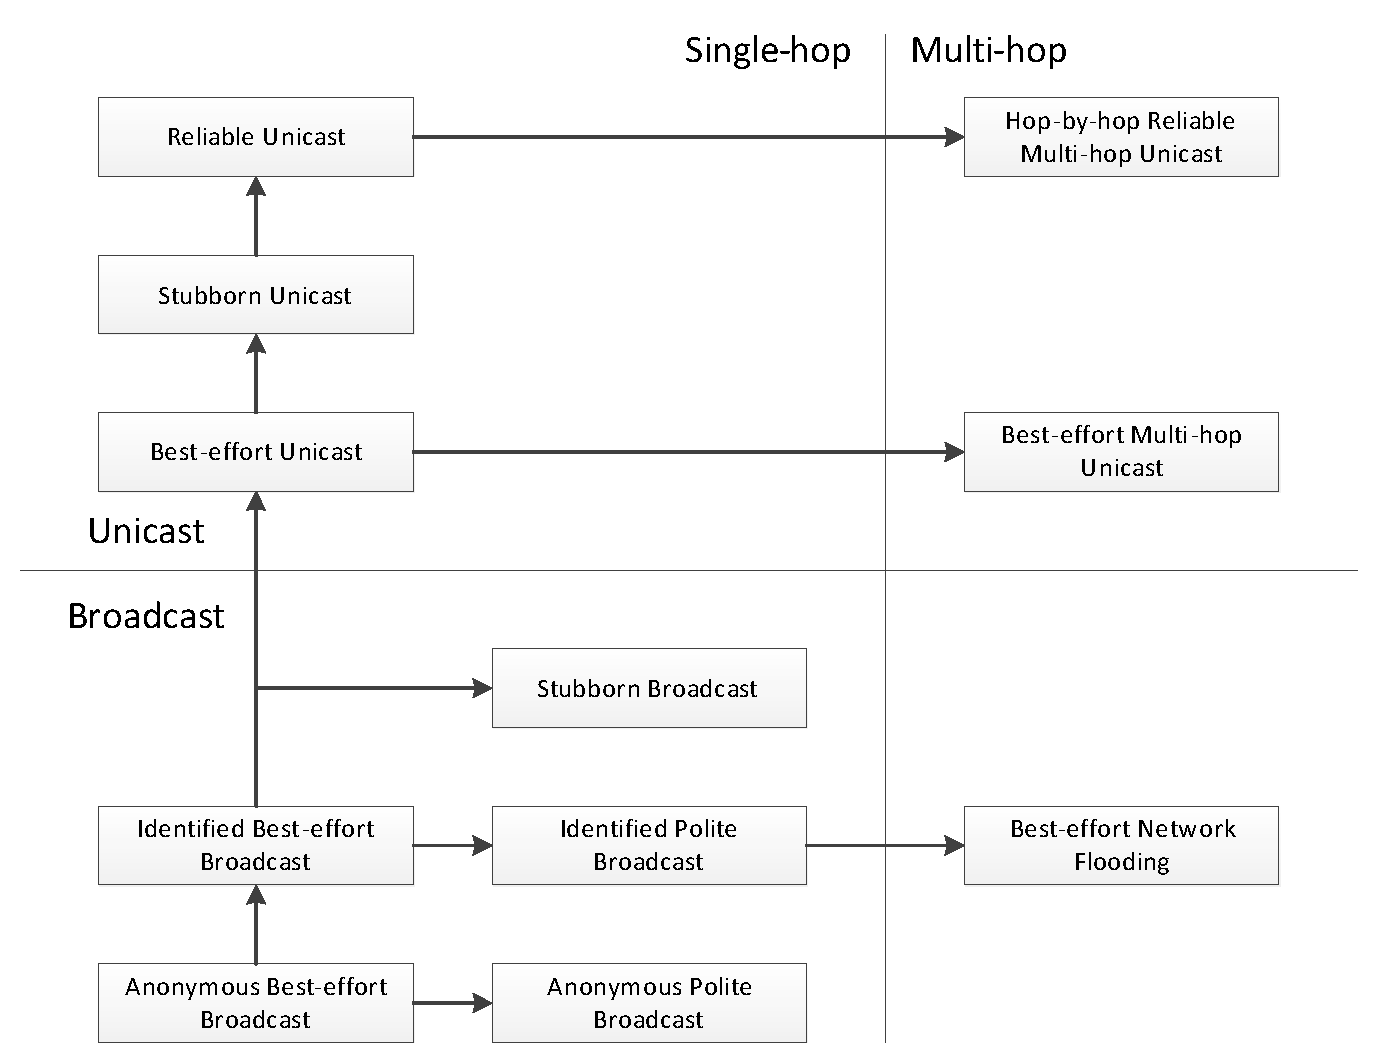
\includegraphics[width=\textwidth]{Diagrams/rime-stack}
	\caption{The communication primitives in the Rime network stack \cite{Dunkels:2007:ACA:1322263.1322295}}
\end{figure}

\begin{table}[H]
	\centering
	\begin{tabular}{ | l | l | l | }
		\hline
		Name & Header & Address \\
		\hline
		Anonymous Broadcast & abc.h & \url{contiki.sourceforge.net/docs/2.6/a01717.html} \\
		Broadcast & broadcast.h & \url{contiki.sourceforge.net/docs/2.6/a01720.html} \\
		Stubborn Broadcast & stbroadcast.h & \url{contiki.sourceforge.net/docs/2.6/a01739.html} \\
		Anonymous Polite Broadcast & polite.h & \url{contiki.sourceforge.net/docs/2.6/a01730.html} \\
		Polite Broadcast & ipolite.h & \url{contiki.sourceforge.net/docs/2.6/a01724.html} \\
		Unicast & unicast.h & \url{contiki.sourceforge.net/docs/2.6/a01738.html} \\
		Stubborn Unicast & stunicast.h & \url{contiki.sourceforge.net/docs/2.6/a01740.html} \\
		Reliable Unicast & runicast.h & \url{contiki.sourceforge.net/docs/2.6/a01738.html} \\
		Network Flooding & netflood.h & \url{contiki.sourceforge.net/docs/2.6/a01728.html} \\
		Multi-hop Unicast & multihop.h & \url{contiki.sourceforge.net/docs/2.6/a01726.html} \\
		Reliable Multi-hop Unicast & rmh.h & \url{contiki.sourceforge.net/docs/2.6/a01732.html} \\
		Reliable Unicast Bulk Transfer & rucb.h& \url{contiki.sourceforge.net/docs/2.6/a00365.html} \\
		\hline
		\hline
		Mesh & mesh.h & \url{contiki.sourceforge.net/docs/2.6/a01725.html} \\
		Collect & collect.h & \url{contiki.sourceforge.net/docs/2.6/a01723.html} \\
		Trickle & trickle.h & \url{contiki.sourceforge.net/docs/2.6/a01742.html} \\
		\hline
	\end{tabular}
	\caption{Communication Primitives headers and documentation location}
\end{table}


\begin{table}[H]
	\centering
	\begin{tabular}{ | l | l | l | l | }
		\hline
		Name & Reliable & Target & Sender Known\\
		\hline
		Anonymous Broadcast & No & 1-hop neighbours & No\\
		Broadcast & No & 1-hop neighbours & Yes\\
		Stubborn Broadcast & No & 1-hop neighbours & No\\
		Anonymous Polite Broadcast & No & 1-hop neighbours & No\\
		Polite Broadcast & No & 1-hop neighbours & Yes\\
		Unicast & No & destination & Yes\\
		Stubborn Unicast & No & destination & Yes\\
		Reliable Unicast & Yes & destination & Yes\\
		Network Flooding & No & network & Yes\\
		Multi-hop Unicast & No & destination & Yes\\
		Reliable Multi-hop Unicast & Yes & destination & Yes\\
		\hline
		\hline
		Mesh & No & destination & Yes \\
		Collect & Yes & destination & Yes \\
		Trickle & Yes & network & No \\
		\hline
	\end{tabular}
	\caption{Communication Primitives behaviour}
\end{table}

\paragraph{Beacon Coordination}
\cite{Dunkels:2011:ALB:1966251.1966270} % http://dunkels.com/adam/dunkels11announcement.pdf

\paragraph{Run-time Reprogramming}
\cite{Dunkels:2006:RDL:1182807.1182810} % http://dunkels.com/adam/dunkels06runtime.pdf

\subsubsection*{NS2}

NS2 is a ``discrete event simulator targeted at networking research'' \cite{NS2} that ``provides substantial support for simulation of TCP, routing, and multicast protocols over wired and wireless'' networks. Due to its initial focus on wired networks the support for wireless networks can be below expectations. NS2 is written in C++ and uses OTcl to manage the simulation of networks. NS2 has a very large number of features, for example many of the routing protocols are built in and it comes with support for mobility models such as random waypoint. Due to the number of features NS2 can be very useful to people who wish to utilise it to its full potential, but it can be difficult to newcomers who may be overwhelmed.

\subsubsection*{JProwler}

JProwler \cite{JProwler} is a Java implementation of Prowler which is implemented in MATLAB. JProwler is designed to simulate MICA motes and provides two radio models: Gaussian and Rayleigh, one is for use with stationary nodes and the other is for use with mobile nodes. The main use case of JProwler is to simulate large networks very quickly. The implementation of algorithms is written in Java, using the simulator as a base, so to transplant the algorithms to run on actual hardware means rewriting the program. The benefits of it are: that it is very fast and it is implemented using Java this enables quick prototyping of algorithms, easy testing and fast analysis.

\subsubsection*{TinyOS}

TinyOS is an event driven wireless sensor network operating system \cite{tinyos}. Programs are written for in nesC a dialect of C \cite{Gay:2003:NLH:780822.781133}. While TinyOS is often described as an operating system it is better described as a framework for developing programs for embedded systems (specifically sensor networks). Developing for TinyOS can be easier than other implementations because the nesC language models that tasks that a developer would be programming a sensor node to be doing better than developing programs directly in C. To simulate applications developed for TinyOS TOSSIM \cite{levis2003tossim} can be used to compile the same nesC code that would be used to run on the hardware to an intermediate format that is understood by the simulator. TOSSIM supports radio models where the bit error rate is configurable and emulates the hardware to provide an accurate simulation of what may occur in a real life situation. Finally the simulator supports visualising the network, so developers can get a good understanding of what is happening.


\subsubsection*{Simulating Energy Consumption}
\cite{Shnayder04}


\begin{comment}
\section{Required Tools}

A simulator and operating system needs to be chosen that will allow us to test our code locally, then provide functionality to deploy that code to the network easily. We will now provide a comparison between the two primary operating systems, Contiki \cite{23839452} and TinyOS \cite{levis2003tossim}, and their respective simulators with a view to deciding which system best suits this projects goals and motivations.

TinyOS and it's simulator TOSSIM were originally created at UC Berkeley as part of the DARPA NEST Program. TinyOS is a static system where designers must allocate resources during design-time. TinyOS is also a monolithic system, in this system programs are compiled with the OS code and distributed to network nodes together as one image.

Contiki was developed by Adam Dunkels and is an open source operating system designed for the Internet of Things. Contiki is a dynamic system that allows resources to be allocated and deallocated at run-time. Contiki is a modular system where programs are compiled into an individual module that can be distributed to the network nodes which run the code dynamically.

Both systems are event driven, however Contiki also offers native multi-threading support through proto-threads where as TinyOS does not and requires a library to gain access to threading through TinyThreads \cite{?}. TinyOS programs are implemented in nesC, a variation of C designed for the TinyOS platform. The simulator COOJA can run both C and Java code but the Contiki OS can only run C code. Both systems use custom wireless networking stacks that are optimised for low power consumption. In a comparison of energy and time efficiency between Contiki and TinyOS \cite{5560028} it is shown that the differences between the two operating systems is negligible. The study found that Contiki is quicker at sensing, TinyOS is faster at communication between nodes and they are both equally efficient at processing tasks such as executing security algorithms.

We have chosen to use Contiki and COOJA for this project because it provides the most flexible system for developing applications that can quickly and easily be distributed to the network. Contiki also offers an easy to use fully functioning development environment and simulator tool all in one package. Finally, Contiki is almost as efficient as TinyOS in nearly every respect but provides all the additional features of a modular dynamic operating system and for these reasons this is why we have chosen it as the system we will develop for. 

\subsection{Risks with Hardware}

With the sensor nodes, we as a group have been given responsibility over them. This means we need to be very careful when transferring then between home and university. We must make sure that they are carried safely, packed away properly and protected from the environment when transferring (for example from rain).

\clearpage
\end{comment}



\subsection{Sensor Network Platforms}

\subsubsection*{MICA}
\cite{Mica2002}

\subsubsection*{Sky}


\subsection{Practical Experience in Sensor Networks}
\label{sec:lit-review-practical-experience}

\subsubsection*{Habitat Monitoring}

Habitat monitoring is widely thought to be one of the key wireless sensor network application that is driving research and adoption. The problem involves determining the location of the sensor nodes, which then allows tracking \cite{Cerpa:2001:HMA:844193.844196} and two of the primary problems in sensor networks: data aggregation and energy efficient multihop communications.

The research undertaken by \citeauthor{SzewczykPMC04} in \cite{SzewczykPMC04} involves deploying sensor nodes on the Great Duck Island in order to test the long term real-world deployment of sensor networks. The importance of deploying and testing a WSN in the real world is due to the fact that challenges are encountered that are not present in indoor deployments or simulations. The problem becomes one of not just what software needs to run and how, but also consider on what hardware in what conditions. For example the authors wished to waterproof the mote in order to ensure that it survived dew, rain and flooding. However, when enclosing the motes it was worried that (i) radio transmissions would be interfered with and (ii) sensor data could be affected.

Overall, the deployed motes performed well (logging 1.1 million readings over 123 days), however, there were a number of abnormal results that included: (i) sensor readings outside their range, (ii) ``erratic packet delivery'' and (iii) failure of motes. The authors point out (in section 2.5) that in the future it would be useful to augment applications with the ability to notify that failures occurred and to perform self-healing.

The performance of the network showed that initially packet loss was up to 20\% but that slowly decreased, most likely due to the fact that the size of the network network was reducing over time (as nodes permanently crashed). Due to the low network utilisation (under 5\%) \citeauthor{SzewczykPMC04} initially believed that collisions would not play an important role, however, their results suggested otherwise. Their results suggest that this was caused by clock drift which lead to slot assignments not preventing collisions within their period. This importance of clock drift on TDMA-based MAC protocols is something that would tend not to be found from testing in a simulator because of the slow speed of simulation and the length of time it takes for these small clock drifts to lead to an effect.

Overall, one of the major conclusions of this work is that anomalous sensor data can be used to predict mote failures with a high degree of accuracy. The authors believe that this prediction allows for a high level of pro-active maintenance, and self-organisation and self-healing of the network.

\subsubsection*{Animal Monitoring}
% https://www.princeton.edu/~mrm/ZNetASPLOS.pdf
% http://citeseerx.ist.psu.edu/viewdoc/download?doi=10.1.1.14.6467&rep=rep1&type=pdf

Instead of monitoring the habitat, why not simply directly monitor the animal in question? This is the track that a number of other wireless sensor networks have taken \cite{Juang:2002:ECW:635508.605408}. The traditional technique was to attach collars that emit radio waves that are used in manual triangulation or take GPS measurements and then recover the hardware attached to the animal to extract the data. Sensor networks provide a way to extract this data automatically in a much easier manner and can also allow for data to be accessed earlier.   Much of what is true for habitat monitoring is also true for monitoring animals: the hardware needs to be protected against the weather, the data needs to be extracted as reliably as possible and the battery should last as long as possible to make the deployment cost effective.

ZebraNet by \citeauthor{Juang:2002:ECW:635508.605408} in \cite{Juang:2002:ECW:635508.605408} investigates these issues as well as some of the unique deployment issues related to mounting hardware on animals. For example it is very important that the hardware is light enough for the animal to handle for a long time. This adds a new type of trade-off, when considering energy usage and reliability system developers must also consider weight.

Aside from the usual issues associated with sensor networks, having sensors attached to animals presents another very important problem that needs to be solved. Many of the animals that we wish to monitor, are desired to monitor for very good reasons. Most often it is the case that they are endangered or are often the victims of poaching \cite{6115161,Biagioni02theapplication}. By attaching wireless devices that broadcast information, it has been found that attackers can trace their way back to a source. There has been much research to develop ways to mitigate this problem, one example is using fake sources to lure an attacker in an alternate direction than that of the real source \cite{Ozturk:2004:SPE:1029102.1029117,Kamat.1437121,6296046}. These additional problems that arise as side-effects of communicating through a wireless medium are often difficult and expensive (in terms of energy) to overcome.

\subsubsection*{Forest Fires}
\cite{libeliumForestFires}
\cite{FireWxNet}
\cite{4428702}
% http://static.usenix.org/events/mobisys06/full_papers/p28-hartung.pdf

While habitat monitoring has been at the forefront of monitoring wildlife habitat and animal behaviour, there is a need to measure and view fire and weather conditions to predict wildland fires that occurs across the globe. Fire behavior can change drastically, depending on different environmental factors and topological features such as elevation and aspect. It is important for such behaviour to be predicted accurately and wildland firefighters are currently using means like observing current weather conditions and weather forcasts provided by the  National Weather Service to do so. While data provided by the weather forcast gives a general overview of fire behaviours, those solely colleted by the firefighters (e.g. using a belt-weather kit) only provides data for a sparse number of regions which is inadequate in making a full evaluation. With wireless sensor networks, firefighters can safely measure weather conditions over a wide range of locations and elevations anywhere withing the fire environment.

FireWxNet by \citeauthor{FireWxNet} in \cite{FireWxNet} is a robust multi-tiered portable wireless system, designed to be deployed in a rugged environment. Compared to other application deployments, FireWxNet covers a unique topology which ranges from substantial and sharp elevation differences to an extremely wide coverage area of about 160 square kilometers. Wide area communication coverage and fine-grained local weather sensing coverage are some of the main challenges that was faced by the team. 

Some of the network challenges was ensuring a high-probability of receiving data from the sensors, regardless of interference and asynchronous links and this was tackled by using a best-effort converge-cast protocol. Other issues included verifying the connectivity between nodes and complications were a result of the sparse nature of the deployment and large chages in elevation between nodes. In addtion, a user could not receive verification when adding a node to a currently depoyed network and required the resetting of a neighbour node to gain connectivity.

When testing the performance of the network, results showed that the networks which were deployed on different mountains obtained an average yield of only 40\% and a 78\% unique yield. This may have been the effect of timing limitations, for example some sensors required some settling time once it was activated before it could produce any accurate readings. The CSMA MAC protocol which would back-off in the presence of interference may have also contributed to the number of packets sent. To improve the sucess rate, they chose the option of resending the packets multiple times, but at the cost of some efficiency. In the future, the team aims at designing protocols such as hop-to-hop ACKS, which hopes to cut down on the number of packet they send. 

\subsubsection*{Structural Monitoring}
\cite{5508230} Claimed: Ivan
% http://ieeexplore.ieee.org/stamp/stamp.jsp?tp=&arnumber=5508230
% Drawbacks on conventional methods: http://www.eecs.berkeley.edu/~binetude/work/report.pdf

GENESI: Green sEnsor NEtworks for Structural monItoring - Structural health monitoring systems for critical infrastructure

Another class of application for wireless sensor networks is the structural health monitoring (SHM) of critical infrastructure such as bridges, tunnels and dams, to estimate the state of structural health or detecting the changes in structure that may affect its performance. The conventional method uses PCs wired to piezoelectrical accelerometers and has drawbacks such as (i) use of long wires over the structure, (ii) high cost of equipment, and (iii) expensive to install and maintain. Since SHM requies high data rate, large data size, and a relatively high duty cycle, it would be more efficient to use a WSN which would provide the same functionality as conventional methods but at a much lower price and permits denser monitoring.

\citeauthor{5508230} in \cite{5508230} developed GENESI or Green sEnsor NEtworks for Structural monItoring, which aims to efficiently harvest and generate energy from multiple-sources with radio triggering capabilities and using new algorithms and protocols to dynamically allocate the sensing and communication of tasks to the sensors. GENESI uses a wide range of electronic such as a power-scalable, high efficiency  DC-DC converters and low-drop regulators as well as different harvesting and power distribution strategies to maximise the provision and collection of energy under a large range of environmental conditions. The system also uses an effective power management strategy to compliment the energy harvester mechanism which improves the battery lifetime up to the theoretical limit.

Besides efficient energy harvesting methods, GENESI also emphasizes on reducing energy consumptions for communication and uses a selective activation scheme to dynamically schedule the activation of a set of passive and active sensors. A task allocation algorithm is used alongisde the scheme to decide which sensors are to be activated and considers factors like node residual energy and field coverage. Chosing the best assignment of the available sensors to task proved a great challenge for the team since this problem involving nodes with radio triggering and harvesting capabilities has never been studied before.

% This article doesn't really talk about the issues faced in the development...

\subsubsection*{Air Pollution}

Air pollution has been a growing concern in congested urban cities as a result of industrialisation and heavy transportation. These concerns include poor air quality and visibility and long term damaging of human health \cite{libeliumAirPollution,wsnpollution}. Traditional methods of air quality monitoring involving quality control stations are expensive and provides low resolution sensing since monitoring stations are less densely deployed. Wireless sensor networks can be used as an urban monitoring system as it has the advantages of being small, easy to set up and inexpensive with real time monitoring capabilities. Sensors which have the ability to measure a wide range of meteorological data such as rainfall, wind speed, temperature, humidity and concentration of pollutants can be deployed in areas of high population density of vehicles and industrial areas. Collected data is transmitted back to the base station via a global system for mobile communication.

\citeauthor{fotuewsnpollution} in \cite{fotuewsnpollution} proposed a Wireless Mesh Network to establish internet connectivity and simultaneously measure air pollution in Sub-Saharan African cities. These cities experience the most problems due to the increase of industry, domestic waste and fuel combustion and that many chemical industries have been established in the central urban areas. However, with poor infrastructure and telecommunication links in Africa, it would be difficult to deploy a sensor network that will measure air pollution since some pollution areas are out of range of the communication service. In addtion, some polluted areas lack the security measures or have industrial restrictions to deploy fixed sensors so they had to use mobile sensors which were attached on vehicles. 

\paragraph{WSN Challenges}

\begin{itemize}
\item Reducing communication interference

High-gain antennas was used to reduce the probability of interference from non-city radio frequency emitters such as WiFi and access points. However, interference may also be caused from inter-device communication and was reduced by using multiple orthogonal channels. Each set of devices would use a unique channel to communicate with a different set of devices for example the mesh network would use a channel Cs with the sensors and channel Cg with the gateway.

\item Limiting number of request messages each sensor can receive from the data server.

The network uses an Ad-hoc On-Demand Distance Vector routing protocol for efficient forwarding of data packets to the data server and makes use of a series of messages to communicate through the network and to discover and maintain data routes. A request message is propagated to the network when the data server requests for a specific data item. All the sensors receives the message and checks whether is it the destination or not. If not, it stores a copy of the message in its buffer containing previously broadcasted request messages and rebroadcasts it back to its neighbours. Once the destined sensor receives the message it sends back a reply message using the reverse path of the data server.

To prevent the sensors from overloading with request messages, each message is set with a Time-To-Live (TTL) value with discards the message when the value expires. This value is dependant on the size of the network where a larger network will have higher TTL value to ensure that the request messages reaches the defined destination.

\item Energy Usage

The wireless mesh network is energy efficient since the sensors are energy constrained. This uses an enhanced energy conserving routing protocol which employs a routing algorithm that aims to distribute data among maximally disjoint paths towards the sink so that the lifeline of the WSN service can be prolonged. It also allows the sensors to participate in carrying the global traffic over the network

\item Data transmission periods

To avoid high energy consumptions, data from the sesors to the data server were only transmitted at specifc times of the day (non-real time). This allowed for energy and bandwidth optimization and thus increasing the network's lifetime on the long run.

\item Optimized placements of mesh router 

Since the network includes mobile sensors, there are chances that it can lose connectivity with the the fixed sensors. A challenge that the team faced was placing the mesh routers in such a way that they were always connected to the mobile and fixed sensors in order to receive the sensed data. This is crucial for network reliability and quality of service.
\end{itemize}

\subsubsection*{Volcano Monitoring}

Active volcanoes need to be monitored to predict the likelihood of future eruptions so that early-warning signs can be issued for the evacuation of habitants near the volcano. Today, volcanoes use wired arrays of sensors such as seismometers and acoustic microphones to collect seismic and infrared (low-frequency acoustic) signals and determining a wide range of factors such as sources of volcanic eruptions, interior structure of a volcano and differentiating eruption signals from noise. A typical study can indlue the placement of several stations around the volcano where each contains a low distribution of wired sensors that collects data to a hard drive. Data is then collected manually in a possibly inconvenient location.

To address the issue of high power consumption of these wired sensors, \citeauthor{Werner-Allen:2006:FYV:1298455.1298491} in \cite{Werner-Allen:2006:FYV:1298455.1298491} introduced the deployment of embedded wireless sensor networks consisting of low-power nodes with minimum CPU, memory and wireless communication capabilities. This allows for long distance real time monitoring of volcanic activities and reducing the need for manual data collection. The main challenge however is that environmental monitoring studies sample at a frequency which is much lower than the sample rate of volcanic time series. This is due to the limited radio bandwidth of the sensors thus requiring the need for efficient power management techniques and accurate time synchronization of the nodes. 

\citeauthor{Werner-Allen:2006:FYV:1298455.1298491} implemented a wireless sensor network that was deployed on the Volcano Tungurahua in central Ecuador using a Mica2 sensor mote platform and three infrasonic microphone nodes. These nodes transmitted data to an aggregation node, which relayed the data over a 9km wireless link to the base station. Time synchronization for the infrasonic sensors was done using a GPS receiver which receives a GPS time signal and relays the data 
to the infrasound and aggregator nodes. Over a period of time, the temperature and battery voltage may change and this may affect the sampling rate of the individual nodes and the precision of the time recorded from the GPS time stamp message. These uncertainties was addressed by applying a linear regression to the logged data stream giving an estimation of the node outputs. In addition, the sensor nodes where required to be protected against harsh environments such as rain and long exposure of sunlight by using waterproof pelican cases and 1/4-wave whip antennas.

Their first deployment on the volcano included a small network where nodes could send continuous signals to each other, however this was not feasible for a larger network deployed over longer periods of time. To solve the issue with bandwidth and energy consumption, the team implemented a distributed event detector which only transmits well-correlated signals to the base station. A local event detection algorithm is used to trigger data collection for uncorrelated signals.

\begin{itemize}
\item Distributed Event Detector

To measure the correlated signal, the distributed detector uses a decentralized voting system among a group of nodes. Each nodes samples data at a continuous rate of 102.4Hz and buffers a window of such data while running a local event detection algorithm. If an event is triggered it uses a local radio broadcast to broadcast a vote to other nodes and a global flood to initiate global data collection from all the nodes. Radio contention is reduced using a token-bases scheme for scheduling transmission, where each nodes transmits their buffer one after the other. 

\item Local Event Detector

The team implemented two local event detectors; a threshold-based detector and an exponentially weighted moving average (EWMA)-based detector. The former is triggered when the signal rises above an upper threshold and below a lower threshold. However due to spurious signals such as wind noise, the detector may be susceptible to false trigger. On the other hand, the EWMA detector calculates two moving averages with different gain parameters and is triggered if the ratio of the two averages and the new sample exceeds some threshold T. This method is less affected by node sensitivity and any duplicate triggers over a window of 100 samples are suppressed.
\end{itemize}

\paragraph{Data Collection and Performance}

During the deployment, the team managed to log 54 hours of continuous data which includes seismoacoustic signals from several hundred events. The raw data was used to analyse the system's performance and many challenges where discovered in the early observations. They discovered that on average only 61 percent of data was retrieved from the network and on several occasions the modems which transmitted data back to the station would experience short drop-outs, causing all data aggregated from the nodes to be lost. In addition, duplicate packets were also recorded as a likely result of redundant retransmission and lost acknowledgement. Both lost and duplicate data had to be accounted for before being stored in the timebase.

\paragraph{Conclusion and Improvements}

In general, the event-triggered model was successful in detecting eruptions and other volcanic events and was able to verify the working of the local and global event detectors by examining the downloaded data. However, since the experiment was deployed over a limited area space of the volcano, further work is to be done to instrument volcanoes at a larger scale. This includes, and most importantly, the management of energy and bandwidth usage of the sensors and increasing its computational power to deviate from continuous data collection to enabling the collection of well-correlated signals. 


\subsubsection*{Power Considerations}


\subsubsection*{Global Predicate Detection}

Perhaps one of the most well known techniques to undertake this kind of debugging is Global Predicate Detection (GPD). GPD involves ``taking a consistent global snapshot of the system and checking whether the snapshot satisfies the global predicate'' \cite{277788}. These snapshots are repeated periodically and checked if they satisfy the predicate, in doing so properties can be detected that are required for the predicate to hold.

However, GPD is not as simple as this. To begin with there are two types of global predicates: stable and unstable. Stable predicates are ones that remain true once they become true \cite{277788} and unstable predicates can fluctuate between true and false. An example of a stable predicate is termination, once a system has terminated it cannot turn it self back on again. There also exists a distinction between strong and weak predicates, where strong predicates hold for the entire network ($definitely : p$) and weak predicates hold for a subset of that network ($possibly : p$) \cite{553309,345831}. Because of the unreliability of wireless networks it may often be the case that all that can be said is that the predicate is possibly true, due to not receiving all the information that is required to evaluate the predicate \cite{?}.


\subsection{Predicate Detection or Checking in Distributed Systems}

\subsubsection*{NodeMD}
\cite{NodeMD}


\subsubsection*{Debugging by Computing Aggregates}
% https://ieeexplore.ieee.org/xpl/login.jsp?tp=&arnumber=1203364
\cite{1203364}


\begin{comment}
\subsection{Quality of Service}
The area of Quality of Service (QoS) within Wireless Sensor Networks (WSN) is largely unexplored, due to the large differences between WSNs and traditional wireless networks. Traditional networks determine QoS based on high bandwidth allowance, as a result of high multimedia demands of applications. WSNs typically do not need to transfer this amount of data, and have a much lower bandwidth because of this. WSNs also have a wide range of different applications, and as a result, it is not clear how to develop transferable approaches to QoS  \cite{Akyildiz2002393}. 

QoS can be reduced to 'a set of service requirements to be met when transporting a packet stream from the source to its destination' \cite{Crawley98aframework}. With traditional networks, redundancy is often introduced to allow for high load/traffic, however redundancy in WSNs can often mean wasted energy usage which is often the main QoS measure in many protocols \cite{AkkayaYounis2003}.

Akyildiz et. al. \cite{Akyildiz2002393} suggested that QoS could be measured in two ways Application and Network. The Application defines measures such as coverage, number of active sensors and exposure, while the Network is concerned with delivering the QoS constrained data, while maintaining network efficiency (minimising resources).

Akyildiz et. al. further went on to describe the challenges specific to WSN; 
\begin{itemize}  
			\item Resource Constraints - Battery life, memory, bandwidth etc
			\item Unbalanced traffic - Traffic flows from large set of sensors into a small set of sink nodes
			\item Data redundancy - The re-transmission of data could result in wasted energy usage
			\item Network Dynamics - Failing nodes/wireless links, energy conservation, mobility etc
			\item Scalability 
			\item Multiple sink nodes - Each node could have a different set of requirements
			\item Packet Critically - Some data may need to flow through the network quicker than other pieces
			\item Multiple traffic types - Different pieces of data flowing through the network at the same time
\end{itemize}

QoS is a difficult term to define, mainly due to its various meanings and perspectives, because of this, measurements of quality must be generated based on the application involved, and the specific requirements of that application.

\subsection{MAC Protocols}

\subsubsection*{Energy-efficient MAC Protocol Designed for WSN for IoT (The submarine paper)}

\cite{6128220} discusses the energy efficiency of existing protocols, including the original adaptation of MAC for WSNs - Sensor MAC (SMAC). Describes the operation of SMAC, which uses a fixed listen/sleep cycle to reduce idle listening time and thus save energy. Goes on to mention two improvements on SMAC: first Timeout MAC (TMAC), in which the listen/sleep cycle is adapted according to network traffic, by means of a simple timeout mechanism; then $\mu$-MAC, which alters between contention and contention-free periods. The former is used to establish network topology and initialise sub-channels (collections of time slots), which are used in the contention-free period to transmit without collisions.

The authors then propose a power-controlled MAC protocol (PC-MAC), which determines the required transmission power level for a packet, thus aiming to save unnecessary energy usage when sending over short distances. This calculation assumes the physical layer of the nodes can transmit frames at one of a discrete set of power levels notified by the MAC layer. Once calculated, the minimum required power for each of a node's neighbours is stored in that node's Schedule and Power Level Table, an extension of the Schedule Table used for synchronising sleep cycles in SMAC. The protocol preserves the collision- and overhearing-avoidance properties of SMAC.
Authors report energy savings of between 50\% and 96\% for average node distances ranging from 10m down to 1m. These findings were generated solely using simulations, but assuming they hold for a hardware WSN the benefits for energy efficiency are significant enough to warrant serious consideration.


\subsubsection*{Energy Analysis of Four WSN MAC Protocols}

Four power-aware protocols based on the MAC framework implemented in TinyOS on TelosB motes and were tested using broadcast, convergecast and local gossip traffic patterns \cite{5751321}. Motivation: testing of the protocols side-by-side under controlled parameters, to rule out the innumerable extraneous factors that make direct comparison of separately-published protocols difficult.

Outlines history of power-saving MAC strategies, beginning with the duty cycles as described above in the operation of SMAC. Then describes the next development --- low-power listening (LPL), using transmission preambles and channel polling to reduce idle listening times. More advanced protocols use a hybrid of these two techniques.

Protocols tested:
\begin{enumerate}
	\item Scheduled Channel Polling MAC (SCP-MAC):
	\begin{itemize}
		\item Modification of LPL by waking up all neighbouring motes to listen at the same time. This leads to shorter preambles and duty cycles than typical LPL protocols (i.e. BMAC). However, all neighbours share a listening slot, so overhearing is common.
	\end{itemize}
	
	\item Asynchronous Schedules MAC (AS-MAC):
	\begin{itemize}
		\item Eliminates overhearing by assigning unique time slots for each mote to listen; the times when each mote wakes up to transmit/receive are determined by its internal Neighbour Table. At each wakeup, a mote polls for packet receptions, and motes transmit during a contention window overlapping with this wakeup slot. Loss of contention signals a retry during the recipient's next wakeup. AS-MAC uses sync packets and non-uniform offsets to offer unique receiver receptions slots, even in dense neighbourhoods.
	\end{itemize}
	
	\item Crankshaft:
	\begin{itemize}
		\item Similar to AS-MAC in that time is divided into frames, which are sub-divided into receiver slots. Frames include broadcast and unicast slots such that all neighbouring motes wake up for the all of the former, and only their own unicast slot. The ratio between the two types of slot is configurable at compile time, and the number of unicast slots is independent of the number of motes. As such, dense WSNs often feature multiple receivers contending for receptions during the same slot; clock synchronization in Crankshaft relies upon upper layers.
	\end{itemize}
	
	\item Broadcastable AS-MAC (BAS-MAC):
	\begin{itemize}
		\item During implementation of broadcasting in AS-MAC (using multiple unicast transmissions), it was noticed that a broadcasting mote must stay awake for the duration of every receive slot in the network; for nontrivial network sizes, this would be infeasible. As such, a separate protocol was created. BAS-MAC is based heavily on AS-MAC, but defines a broadcast interval; a time slot during which all neighbouring motes wake up simultaneously.
	\end{itemize}
\end{enumerate}

Measurement of the energy usage of each protocol was approached by recording the amount of time motes spent in each radio state, and multiplying each of these times by a constant representing the energy usage of that state per unit time. These constants were determined using an oscilloscope connected to a mote running AS-MAC (as energy consumption per state is protocol-independent). Minor alterations were made to each protocol to  ``level the playing field" in the case of slow/complex protocol initialisations and inapplicable network assumptions.

The results of the experiments, organised by network traffic type, are as follows.
\begin{enumerate}
	\item Local gossip:
	
	AS-MAC demonstrated highest energy efficiency for this traffic type, with Crankshaft and BAS-MAC both using approximately 40\% more energy (due to increased idleness caused by the lack of broadcasts), and SCP-MAC using more energy still due to its overhearing avoidance being inapplicable due to the packet-based TelosB motes.
	
	\item Convergecast:
	
	AS-MAC shows the best overall performance again, though for receiving motes the energy usage of SCP-MAC is a very close second. Again, the unused second wakeup for Crankshaft and BAS-MAC leads to idling.
	
	\item Broadcast:
	
	As AS-MAC is inherently poorly suited to broadcasts, its sender used almost triple the energy of that of the next-least efficient protocol, though its receivers were most efficient by a small margin. Thus, in a single-hop network where the base station node is not battery powered, it is a good choice. However, SCP-MAC performed best overall, by a significant margin over both Crankshaft and BAS-MAC.
\end{enumerate}

The authors conclude that no single protocol excels in all circumstances; AS-MAC and SCP-MAC are more efficient with non-broadcast and broadcast traffic, respectively, where BAS-MAC performs moderately well in each scenario. However, as the base station for our network will typically be a laptop or desktop, the disadvantage of AS-MAC in broadcasting could potentially be ignored. The authors also suggest using a framework such as MLA to host a suite of protocols suited to different tasks, each of which may be swapped in to match the current circumstances.

This last point may well prove to be beyond the scope of our project, however the results for individual protocols may prove useful. It is unfortunate that a fair comparison between these protocols and PC-MAC could not be made.

\subsubsection*{A Traffic Queue-aware MAC Protocol for WSNs}

This paper \cite{4469515} introduces the traffic Queue-aware Sensor MAC protocol (QSMAC), based on SMAC to predict amount of data traffic in a network.

After describing the operation of SMAC (as above), the authors highlights the problem of a fixed cycle duration in networks where traffic loads can fluctuate; an overflowing node buffer queue may cause packets to be discarded, causing additional energy expenditure in resending lost packets and debasing the network QoS.

The basic operation of QSMAC involves examining the average increase rate of data packets in a node's buffer queue. When this rate is more than one per second, packets are arriving faster than they can be processed using the default SMAC cycle, so the cycle duration is halved to double its effective processing speed. When the buffer is almost empty, the default cycle is restored.

Simulations show performance greater than that of SMAC in terms of packets' delay, energy consumption, packet reception ratio and network throughput. As above, if these benefits translate to real hardware, QSMAC potentially offers a real improvement over existing wireless MAC protocols. However, its use in our network will have to be carefully considered, as it is currently unknown whether fluctuating traffic loads will be a likely scenario.
\end{comment}
